\documentclass[]{article}
\usepackage[T1]{fontenc}
\usepackage[pdftex]{graphicx}
\graphicspath{ {./img/} }
\usepackage{graphicx}
%opening
\title{Book shop}
\renewcommand{\figurename}{Rys.}
\author{Kacper Wójcik, Marcin Stefaonwicz, Paweł Nowak}

\begin{document}

\maketitle

\begin{abstract}
	Book shop jest projektem sklepu internetowego z książkami. Głównym założeniem było stworzenie platformy przy użyciu Spring Boota z Mavenem, która pomoże użytkownikom w prowadzeniu sklepu internetowego. Przy użyciu dockera powastał kontener zawierający bazę danych PostgreSQL. React razem z Vite, odpowiedzialny jest za warstwę, którą bezpośrednio odbiera klient tj. warstwę frontu, z której dane są odbierane od klienta i wysyłane po przez REST API na część backendową, oraz do której są wysyłane informacje z serwera.

\end{abstract}
\section* {Inicjalizacja}
Aby móc uruchomić projekt trzeba:
\begin{itemize}
	\item zainstalować dockera
	\item sklonować zdalne repozytorium https://github.com/KWojcik243/SKE-FB-Book-shop
	\item wejść do folderu z projektem
	\item użyć komendy \textbf{docker-compose up --build}, aby zbudować pustą bazę
	\item w programie do uruchamiania kodu, odpalić plik "SKE-FB-Book-shop$\backslash$src$\backslash$main$\backslash$java$\backslash$com $\backslash$example$\backslash$demo$\backslash$SkeFbBookShopApplication.java"
	\item zainstalować nodeJS
	\item w folderze SKE-FB-Book-shop$\backslash$fronten$\backslash$bookshop-frontend w terminalu użyć:"npm install" a następnie "npm run dev"
\end{itemize}

\newpage

\section{Projekt systemu}
\begin{figure}[h]
	\centering
	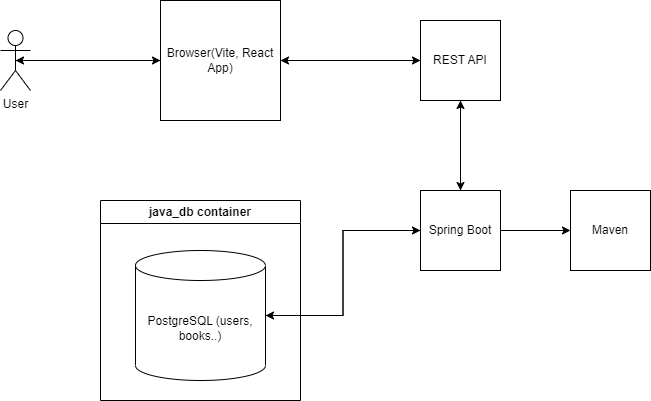
\includegraphics[scale=0.45]{ogolny_projekt.png}
	\caption{Ogólny projekt systemu}
\end{figure}
\subsection{Spring App}
Przy użyciu spring boota budujemy główną aplikacje i inicjujemy możliwość przepływu danych po przez np. REST API.
Dodanie tokena JWT umożliwiło nam w sposób bezpieczny przesyłanie na do przeglądarki informacji o tym jaki użytkownik jest zalogowany, oraz jego prawa dostępu.

W tym projekcie został użyty Maven służący do kompilacji i budowania projektu, oraz do dodawania nowych zależności do frameworku.

Przy użyciu Spring Boota w wersji 3.0.6 został stworzony projekt ze starterów m.in. jdbc, webmvc-ui.

API posiada wiele endpointów, które używane są do tego, aby umożliwić odbiór informacji z frontu, oraz aby móc wysłać na niego niezbędne dane.
Wszystkie endpointy dostępne są do sprawdzenia po odpaleniu projektu na stronie http://localhost:8080/swagger-ui/index.html


Używanie swaggera ułatwia pracę na wielu punktach końcowych, które przy skali projektu i ich ilości mogły by być ciężkie do zrozumienia bez odpowiedniej dokumentacji, a nawet wtedy swagger jest nie zastąpionym narzędziem do testowania tych endpointów.


\subsection{React}
Aplikacja którą odbiera klient została napisana w reacie przy pomoce Vite. Najważniejszymi stronami są:
\begin{itemize}
	\item http://127.0.0.1:5173/dashboard, gdzie Admin może dodawać książki, edytować je, usuwać, dodawać adminów itp 
	\item http://127.0.0.1:5173/catalog, pozwala przeglądać książki i dodawać je do koszyka
	\item http://127.0.0.1:5173/basket, pozwala na składanie zamówień.
\end{itemize}

\subsection{PostgreSQL}

  Kontener stworzony w docker-compose przechowuje i pozwala zarządzać bazą danych PostgreSQL. Została wystawiona na port 5433, aby umożliwić wymianę danych między nią i spring bootem, a jej zabezpieczenia np. możliwość stworzenia indywidualnych kont, oraz haseł pozwala zachować nam względne bezpieczeństwo. PostgreSQL został wybrany ze względu na jego popularność, szybkość działania, oraz to, że jest oparty na modelu relacyjnym.
Baza danych zawiera w aktualnej formie 8 tabel, którymi są:
\begin{itemize}
	\item users
	\item authors
	\item orders
	\item order\_items
	\item books
	\item book\_categories
	\item cart\_items
	\item cart
\end{itemize}
\begin{figure}[h]
	\centering
	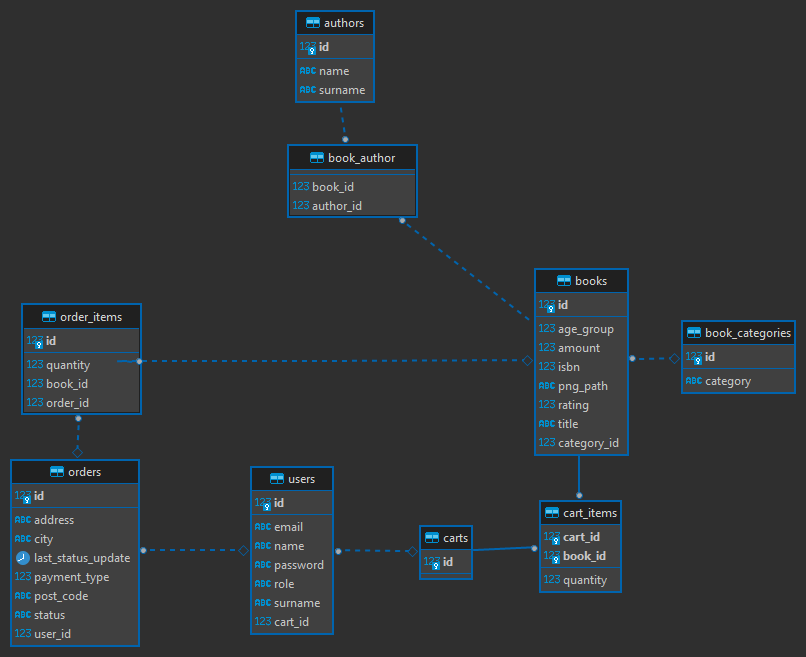
\includegraphics[scale=0.45]{../../postgres.png}
	\caption{Projekt bazy danych}
\end{figure}
\newpage

\subsection{Przypadki użycia}

\begin{figure}[ht]
	\begin{minipage}{\textwidth}
		\indent Stworzony diagram przypadków użycia (Rys.3), przedstawia w sposób ogólny interakcje z aktorem(Userem), ramy systemu, oraz przypadki użycia. Użytkownik może stworzyć konto, zalogować się, przeglądać książki, a następnie po zalogowaniu zarządzać koszykiem tj. dodawać i usuwać książki z niego, lub przystąpić do zakupu.
	\end{minipage}
	\vspace{15pt}
	
	\centering
	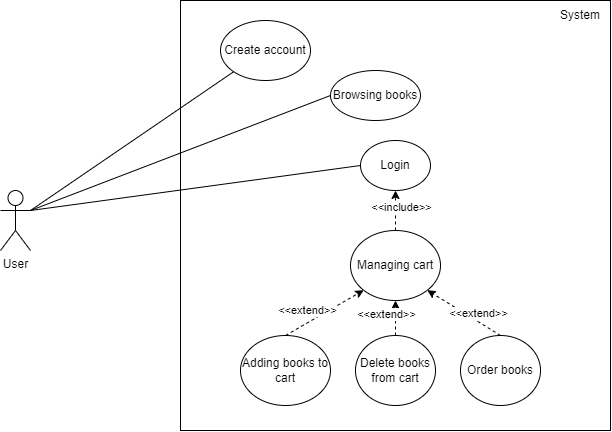
\includegraphics[scale=0.50]{przypadki_uzycia.png}
	\caption{Diagram przypadków użycia - User}
\end{figure}

\begin{figure}[ht]
	\begin{minipage}{\textwidth}
		Diagram przypadków użycia(Rys.4 Admin), przedstawia interakcje z aktorem(Adminem). Aktor może założyć konto, przeglądać książki. Po zalogowaniu dostaje możliwość zarządzania zamówieniami tj. zmiana statusu, realizacja itp., zarządzanie książkami, oraz nadawanie i odbieranie statusu admina innym użytkownikom.
	\end{minipage}
	\vspace{15pt}
	
	\centering
	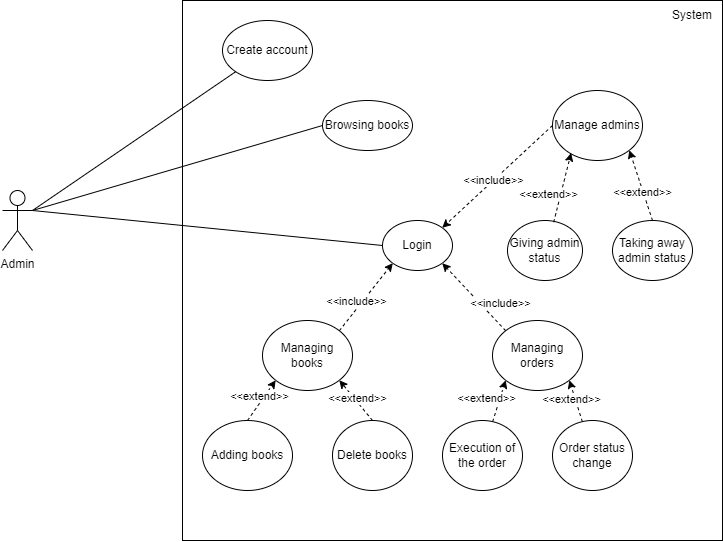
\includegraphics[scale=0.50]{przyp_uz_admin.png}
	\caption{Diagram przypadków użycia - Admin}
\end{figure}

\begin{figure}[ht]
	\begin{minipage}{\textwidth}
		Diagram aktywności logowanie/rejestracja(Rys.5) pokazuje proces rejestracji nowego użytkownika oraz proces logowania dla istniejących użytkowników. Zawiera weryfikację danych, oraz tworzenie konta użytkownika.
	\end{minipage}
	\vspace{15pt}
	
	\centering
	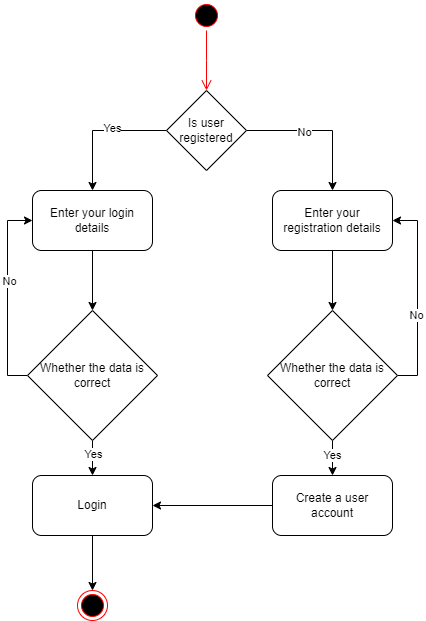
\includegraphics[scale=0.50]{log_rej.png}
	\caption{Diagram aktywności - logowanie/rejestracja}
\end{figure}

\begin{figure}[ht]
	\begin{minipage}{\textwidth}
		Diagram aktywności zakup książek(Rys.6) obejmuje kroki, które użytkownik podejmuje, aby dokonać zakupu książki. Obejmuje to wyszukiwanie książki, dodawanie jej do koszyka, przeglądanie koszyka, podawanie informacji o dostawie, wybór metody płatności, finalizację zamówienia itp.
	\end{minipage}
	\vspace{15pt}
	
	\centering
	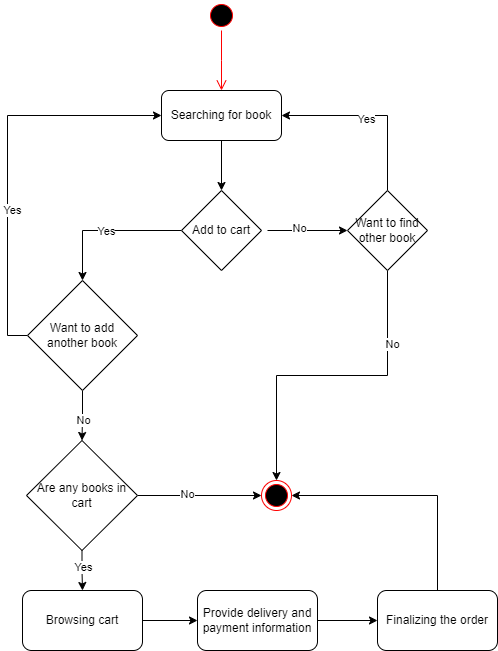
\includegraphics[scale=0.50]{zakup_ks.png}
	\caption{Diagram aktywności - zakup książek}
\end{figure}


\begin{figure}[ht]
	\begin{minipage}{\textwidth}
		Diagram aktywności obsługa zamówień(Rys.7), skupia się na obsłudze zamówień po ich złożeniu. Obejmuje głównie akcje zmiany statusu, oraz wysyłki.
	\end{minipage}
	\vspace{15pt}

	\centering
	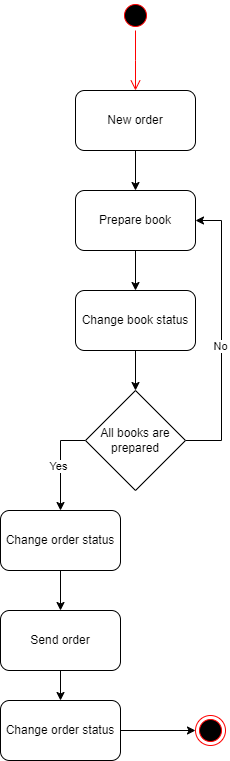
\includegraphics[scale=0.50]{obsl_zam.png}
	\caption{Diagram aktywności - obsługa zamówień}
\end{figure}





\end{document}
